\chapter{Analysis Improvements}
\label{analysis_improvements_overview}

\par The analyses described in the previous two chapters use
sophisticated multivariate analysis (MVA) techniques to perform signal
extraction and limit setting.  However, there are several improvements
that can still be made to optimize signal extraction and increase
sensistivity.  The following section will describe the implementation
of the latest simulation techniques in order to improve the modelling
the signal and background processes.  The final section will discuss
variables from these new simulations that can be used to enhance the
identification of final state jets with their roles in the \ttbar
system.   


%\section{Selection and Category Optimization}
%\label{selection_and_cateogry_optimization_overview}
%
%\par After unblinding, and limit setting, there is an \textit{a
% posteriori} opportunity to study the event selection and
%cateogrization with respect to the ublinded data.  The effects of
%loosening the jet and lepton \PT thresholds, down to 25 \GeV, showed
%improvement in the observed limits.  However, when the limits with
%this new selection were performed in a blinded manner, the expected
%limit did not show the same improvements.  



\section{aMC@NLO, MadSpin, and Pythia8 Monte Carlo}
\label{aMCatNLO_pythia8_overview}

\par One of the largest sources of uncertainty in each analysis comes
from the theoretical uncertainty of the Leading Order (LO) monte carlo
sample  used to estimate background rates and shapes.  In order to
accurately model the high jet-multiplicity environment of the \ttH
final state, higher-order calculations in perturbation theory are
necessary.  Recently, the aMC@NLO framework has been released, and is
an automated tool for event generation that utilizes Next-to-Leading
Order (NLO) QCD predictions \cite{Alwall:2014hca}.  This framework
takes advantage of recent theoretical developments in the automation
of calculating spin-entangled decays from heavy resonances, which is
packaged in the program MadSpin \cite{Artoisenet:2012st}.  The event
generator, aMC@NLO, using MadSpin to calculate the decays of the top
quark, $W$ and $Z$ bosons, is then interfaced to Pythia 8 to framework
perform the parton shower and hadronization \cite{Sjostrand:2007gs}.
Each stage of this event generation process uses the latest
technological developments in monte carlo simulation, which were
unavailable at the time of the previous analyses.  

\par For process where additional jets are simulated in the final
state, there will be an additional complication since the parton
shower and hadronization are performed separately and the
contributions for NLO processes will be double counted in several
cases.  This occurs when a process with an additional jet in the final
state is created in the matrix element level by aMC@NLO and later,
another event is created with no additional jets in the final state at
the matrix element level, but when the parton shower occurs in Pythia
8, an additional jet can be generated, creating two event from a
single underlying theoretical contribution.  The removal of these
overlapping events is carried out by a method known as FXFX
merging \cite{Frederix:2012ps}.  This alorithm tracks the heritage of
final state jets, in order to determine whether it was created as part
of the matrix element or later during the parton shower.  Due to the
higher accuracy of modeling the kinematics of partons calculated in
the matrix element stage, the algorithm removes events where
additional jets are created in the parton shower, ensuring that the
underlying process with an additional final state jets are created
at the matrix element level, utilizing the NLO QCD calculations in
aMC@NLO.  

\par The utilization of these event generation techniques to simulate
\ttH and \ttjets backgrounds will improve the kinematic modeling of
these high-jet multiplicity processes.  A dedicated \ttbb sample with
a large number of events generated with this framework would improve
the modelling of the irreducible background.  Unfortunately, these
event generation tools were only recently released and the
computational time required to generate samples with the equivalent
statistical power of those used in the previous analyses is
prohibitive on the time scale of this dissertation.  However, each of
the following samples were created using the process described above
with 500,000 events each: 

\begin{itemize}
  \item \ttbar + 0, 1, and 2 addtional jets
  \item \ttbb
  \item \ttH + 0, and 1 addtional jets
\end{itemize}

\noindent The number of events generated is not sufficient to create a
control region to asses calibrations of jet energy, $b$-tag
efficiency, or lepton identification and reconstruction efficiency.
However, since all of these processes are generated in an identical
framework, it is reasonable to assume that calibrations applied will
be similar for each, and as such comparisons amongst the samples can
still provide insight into how they can be used to improve the
analysis.  Figure \ref{fig:aMCatNLO_nJets_nTags} shows a comparison
between the number of reconstructed jets and $b$-tagged jets that pass
the selection used in the previous analysis, with a lowered \PT
threshold of 25 GeV.  As before, the jet multiplicity of \ttH has a
much longer distribution than the \ttjets backgrounds, making it very
important that these high-multiplicity events are modeled with the
highest precision available.  

\begin{figure}[hbtp] 
  {\centering
    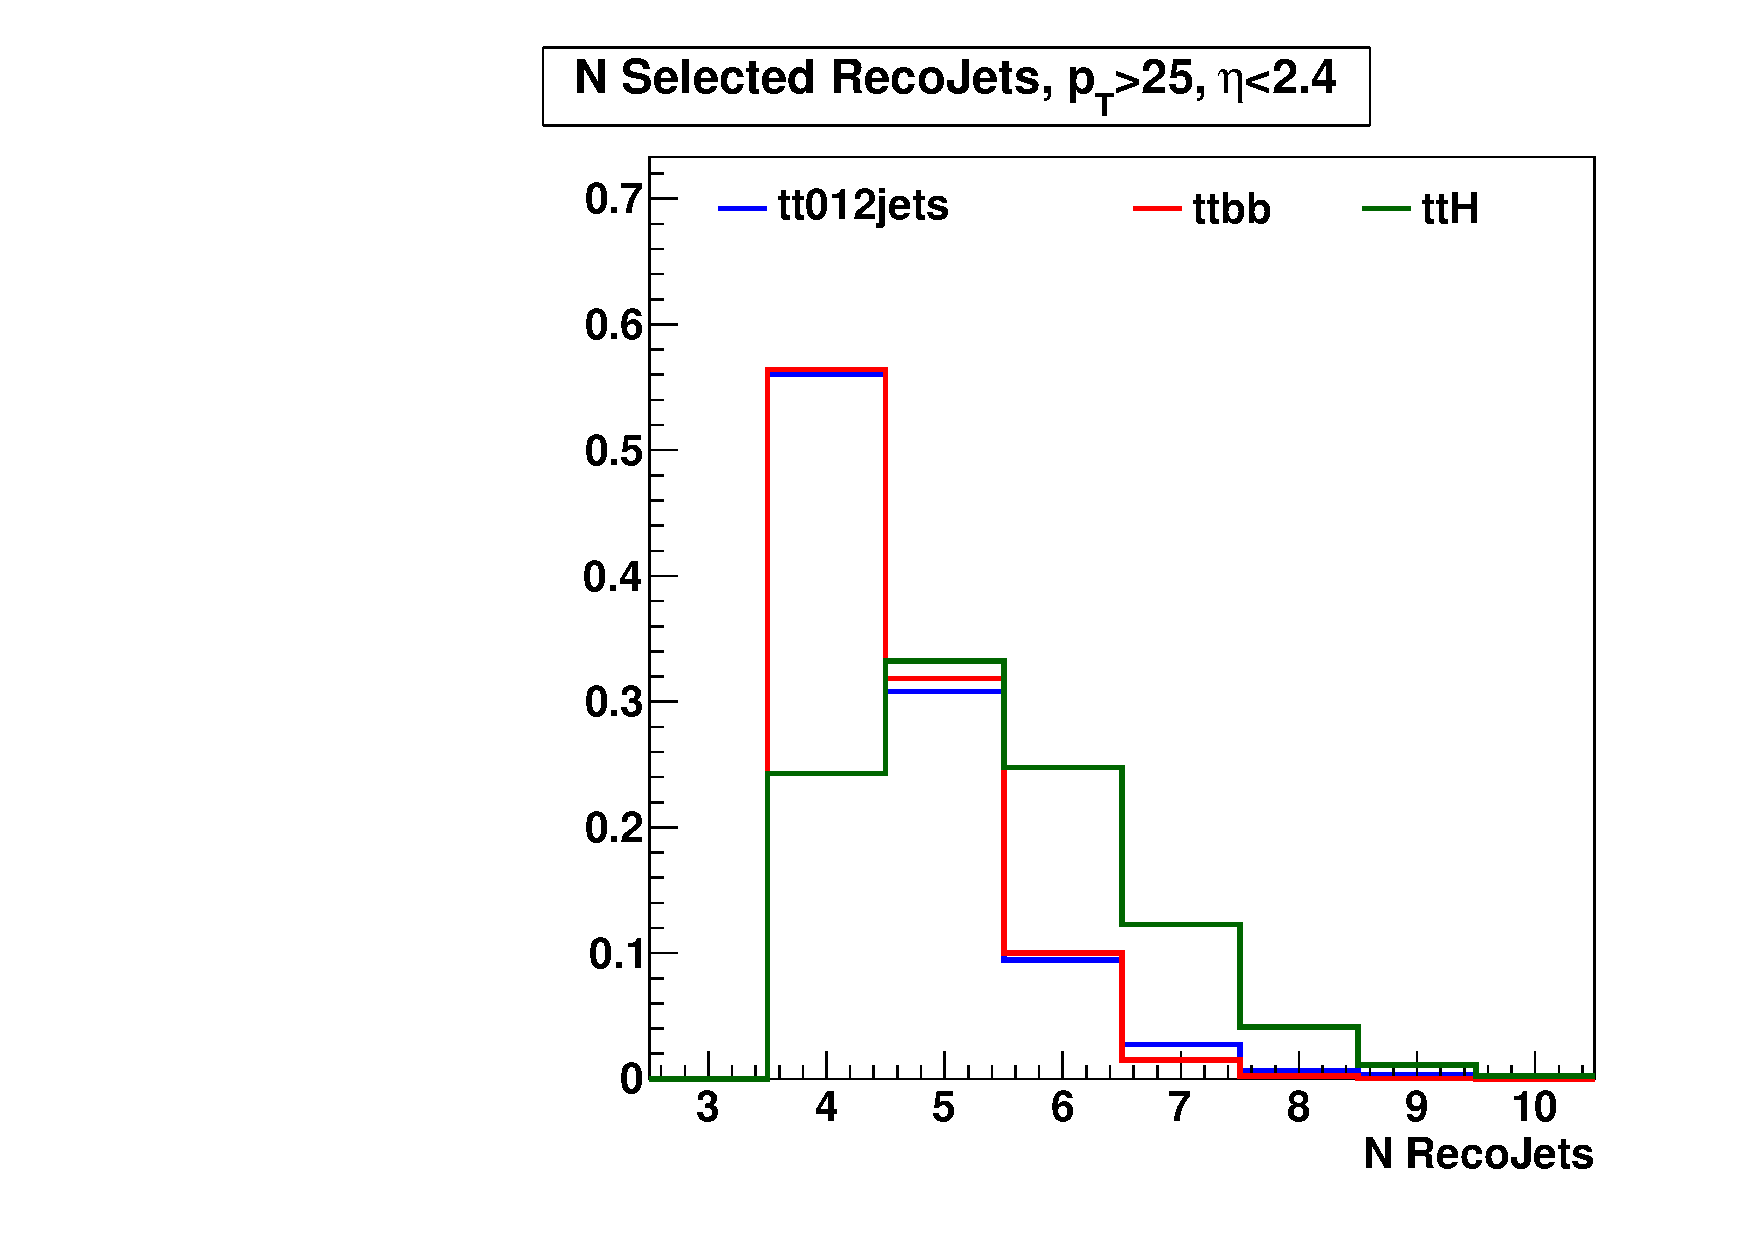
\includegraphics[width=0.48\textwidth]{Figures/Analysis_Improvement_Diagrams/tt012jets_ttbb_ttH__h_recoJet_nRecoJets__unitNorm.pdf}
    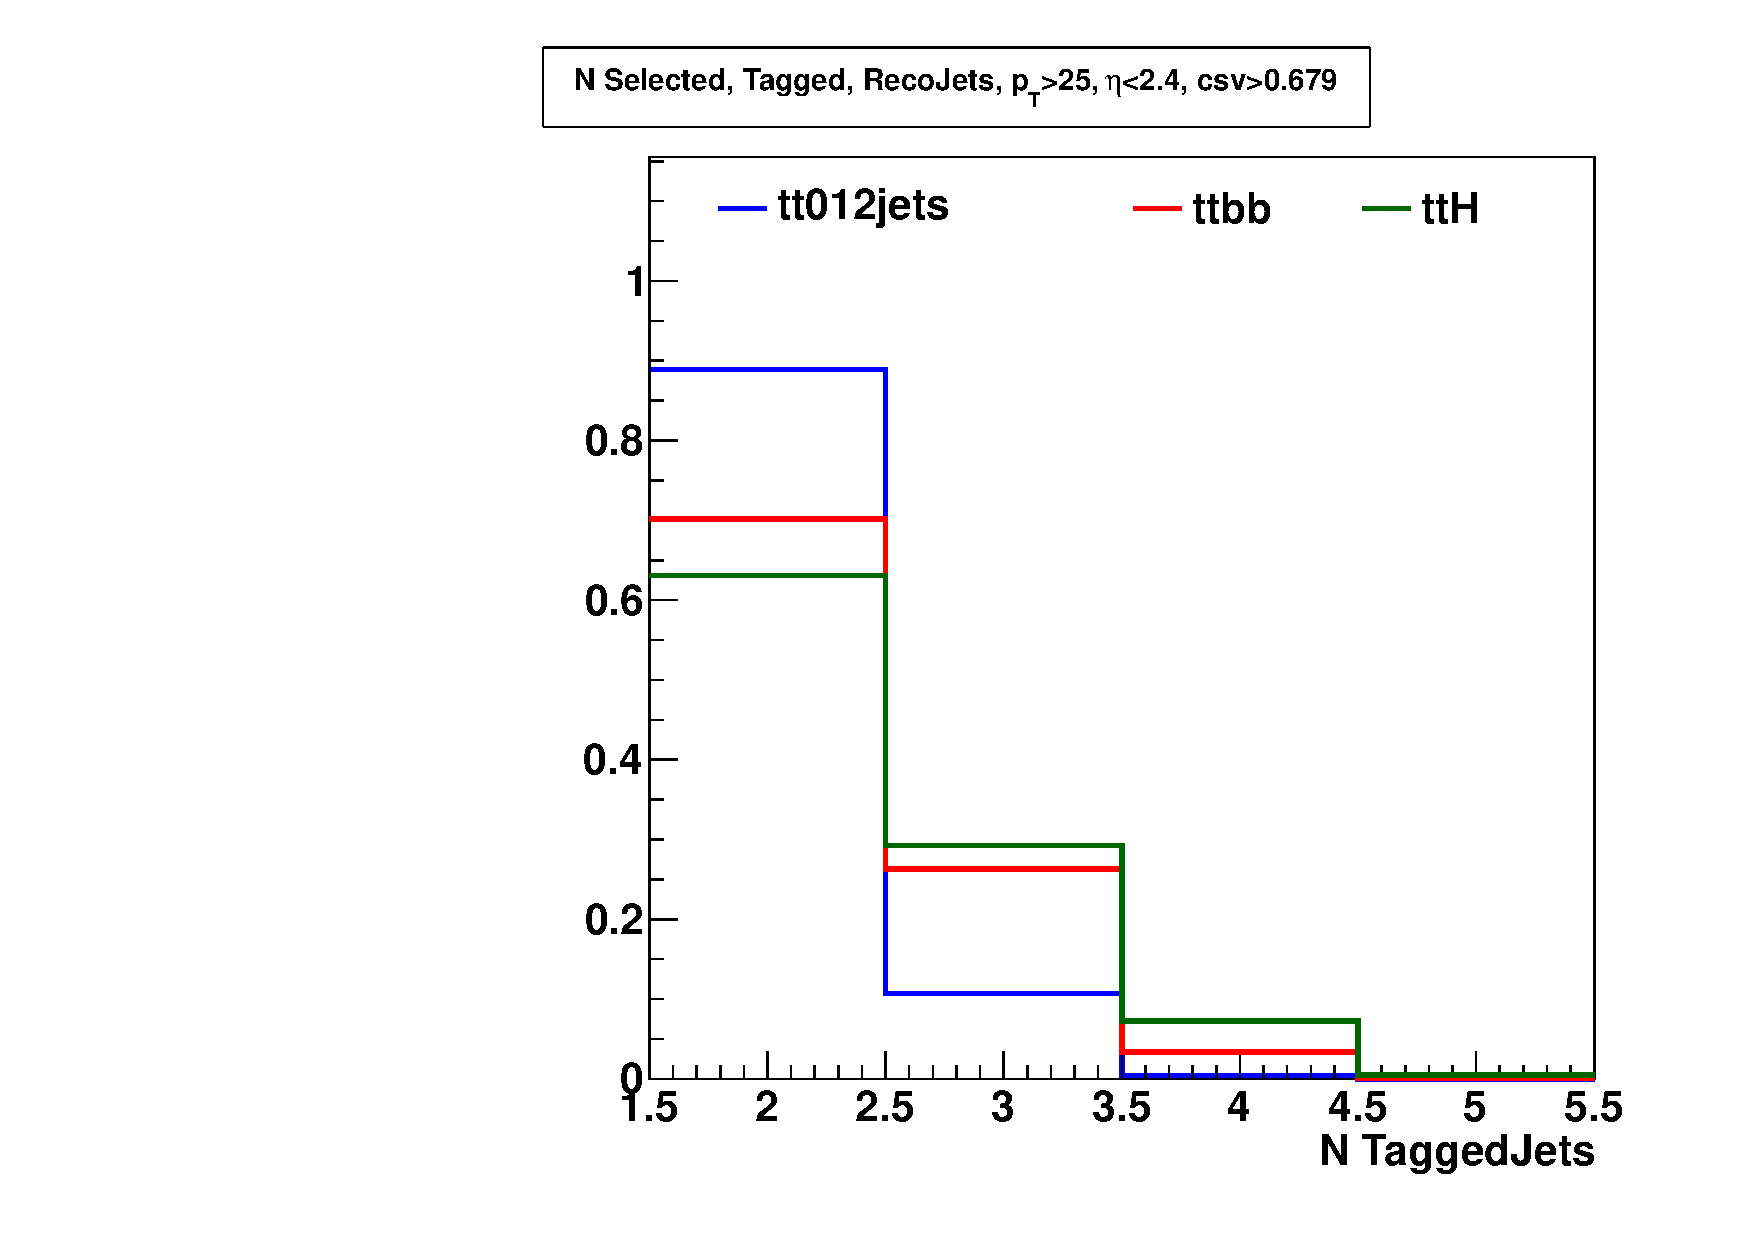
\includegraphics[width=0.48\textwidth]{Figures/Analysis_Improvement_Diagrams/tt012jets_ttbb_ttH__h_recoJet_nRecoTaggedJets__unitNorm.pdf}
    \caption{The number of reconstructed jets passing selection (left)
    and that have additionally been $b$-tagged (right) for \ttH,
    \ttjets, and \ttbb samples generated with the aMC@NLO and Pythia 8
  framework}
    \label{fig:aMCatNLO_nJets_nTags}}
\end{figure}

\section{Analysis Techniques Under Development}
\label{analysis_techniques_overview}

\par One of the most difficult challenges of the \ttH final state is
the combinatorics of possible $b$-jet candidates coming from the Higgs
decay.  The correct associate of jets to their roles in the decay of
the top quarks would greatly reduce the number of jets as candidates
for Higgs daughters.  This is done, in some degree, in the analyses
described in previous chapters via the "best Higgs mass'' variable.
This is a $\chi^{2}$ minimization that relies only on the masses of
the top quark, $W$ and Higgs bosons in the event, to decide which jets
are associated to the decays of which particles.  These mass variable
will be useful in identifying jets from the \ttbar system.  Figure X shows the
case for the $W$ boson mass evaluated for jets which have been
correctly associated to the MC truth generated partons in blue, and
for the incorrect associations in green.  

\begin{figure}[hbtp] 
  {\centering
    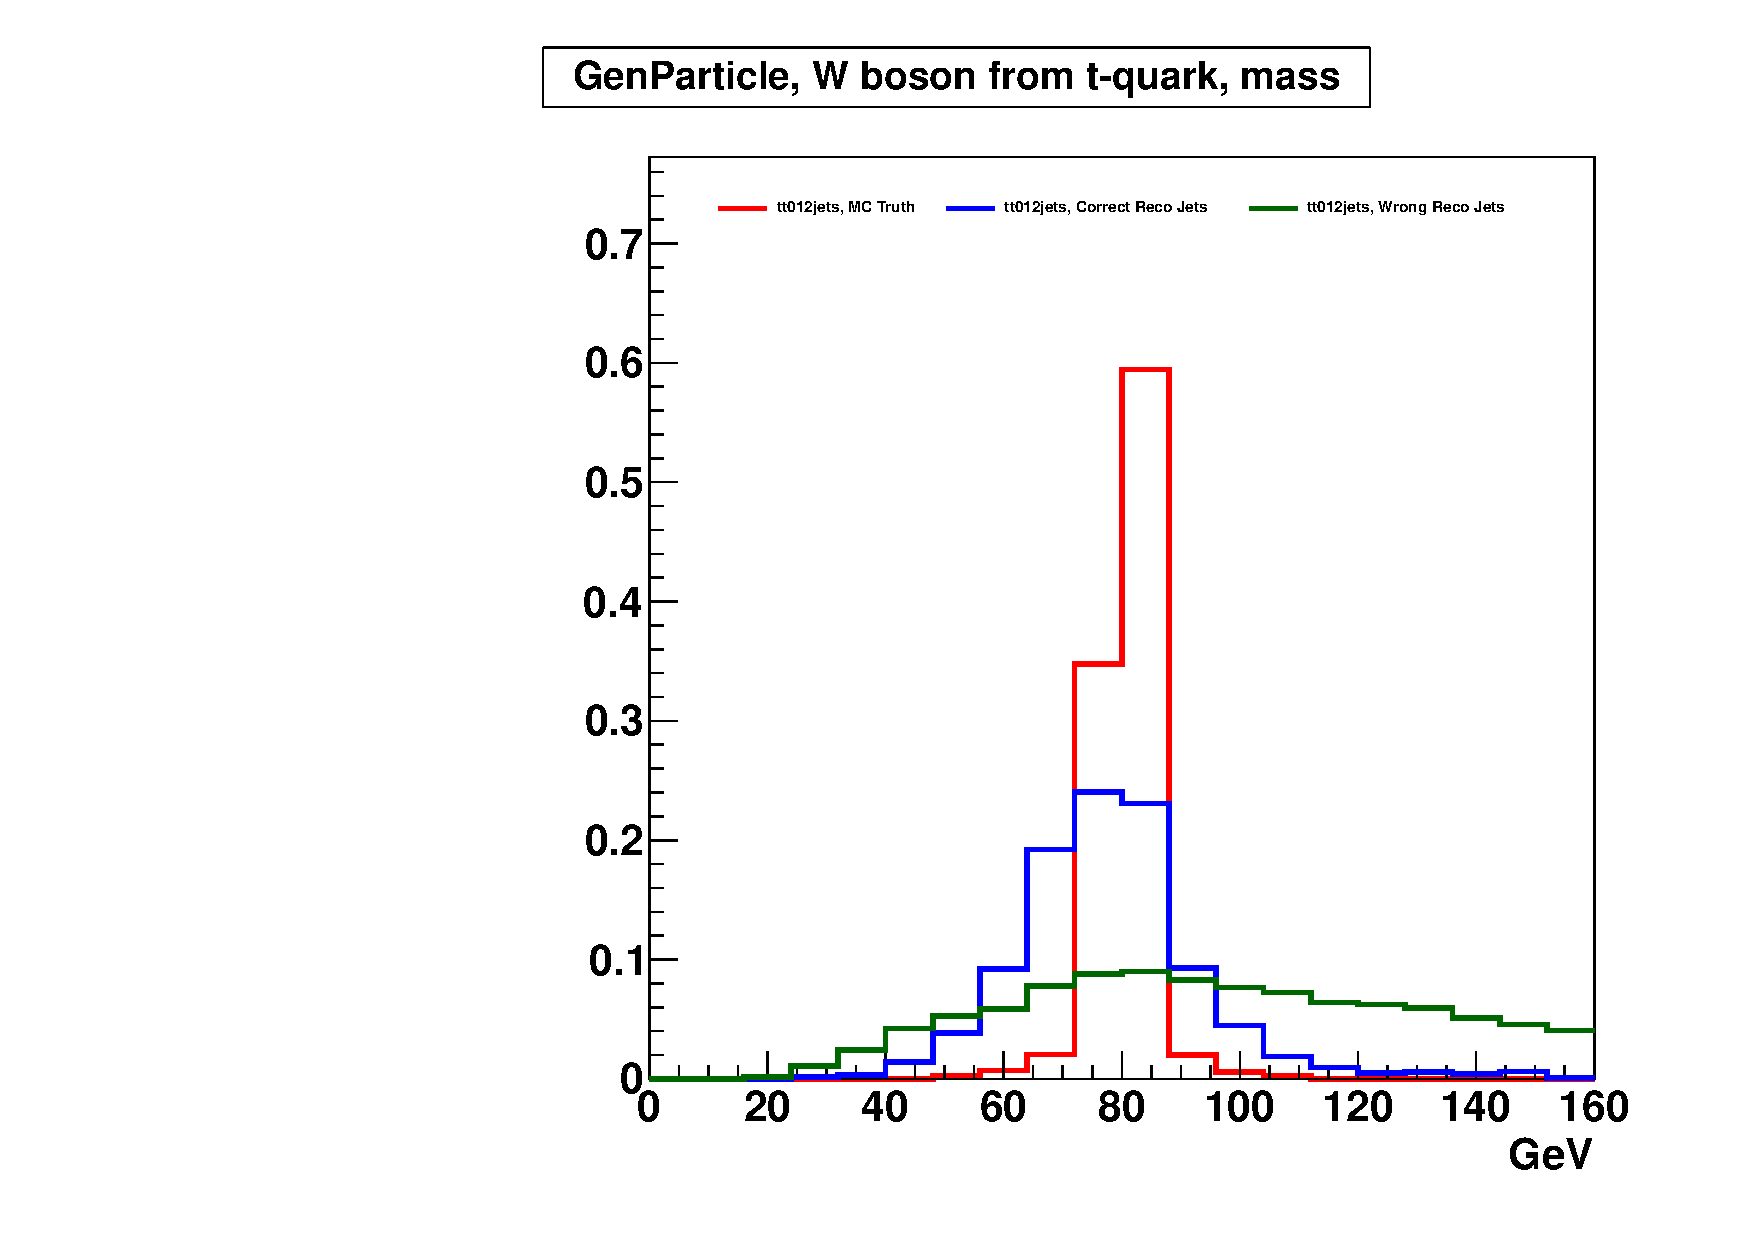
\includegraphics[width=0.50\textwidth]{Figures/Analysis_Improvement_Diagrams/tt012jets__h_genParticle_w_boson_fromTop_mass__vs__h_recoJets_correctAssoc_labFrame_mHadW__vs__h_recoJets_wrongAssoc_labFrame_mHadW__unitNorm.pdf}
    \caption{The invariant mass of the $W$ boson in the \ttbar decay
      for the case of the MC truth (red), correctly associated reconstructed
      jets (blue), and incorrectly associated reconstructed jets (green)}
    \label{fig:aMCatNLO_wMass}}
\end{figure}

\par The implementation of Madspin in the aMC@NLO framework allows for
the highest precsion on the spin correlations of the decay
products from the \ttH and \ttbar systems.  The angular relationships
among the decay products provide additional discrimition power for the
correct association of jets to their roles in the \ttH and \ttbar
systems.  The spin correlations of the decay products are enhanced by
boosting to a reference frame that is more sensitive to differences in
the angles between the correctly and incorrectly associated objects in
the event.  The reference frame of choice is formed by first
identifying all of the potential candidates of the semi-leptonic
\ttbar decay:

\begin{itemize}
  \item $\bar{b}$-quark coming from the $t$-quark
  \item $b$-quark coming from $\bar{t}$-quark
  \item up-type quark from hadronic $W$ boson decay
  \item down-type quark from the hadronic $W$ boson decay
\end{itemize}

\indent The four-vector of the entire \ttbar system can be formed, and
the hadronic candidates are boosted to a frame where the \ttbar system
itself is at rest.  Then, the $t$-quark, and its daughters are boosted to
a frame such that the $t$-quark is at rest.  Finally, the
$\bar{t}$-quark, and its daughters are boosted to a frame such that
the $\bar{t}$-quark is at rest.  Then the angles between their decay
products is evaluated.  Typically, these studies are performed in the
di-lepton channel since the angular resolution is much better in
leptons than in jets.  Figure \ref{fig:aMCatNLO_cos3dPolar} shows the
cosine of the momentum 3-vector between the $b$-quarks from $t$ and
$\bar{t}$, the lepton and the up-type $W$-boson daughter, and the
lepton and the down-type $W$-boson daughter.   

\begin{figure}[hbtp] 
  {\centering
    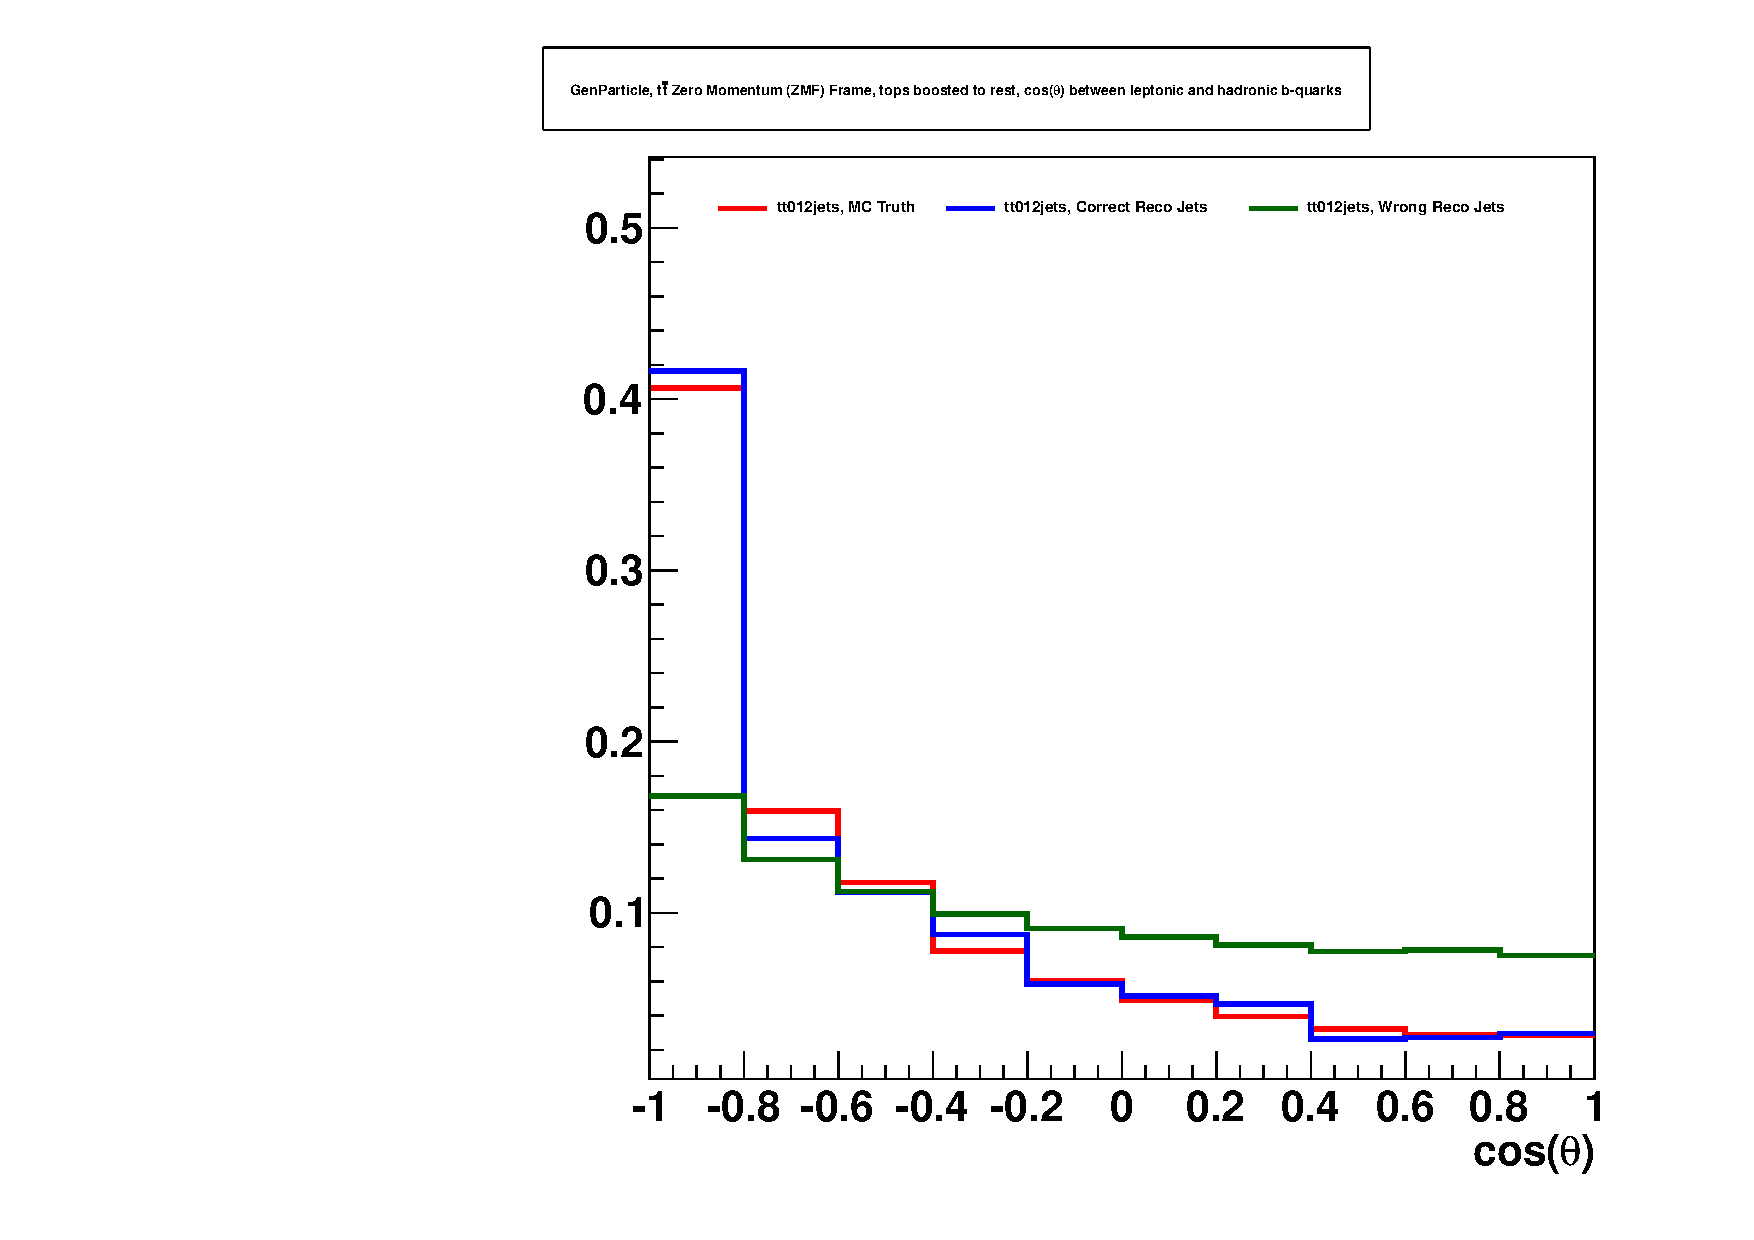
\includegraphics[width=0.31\textwidth]{Figures/Analysis_Improvement_Diagrams/tt012jets__h_genParticle_ttbarZMFrame_topsRest_cos3dPolarAngle_lepB_hadB__vs__h_recoJets_correctAssoc_ttbarZMFrame_topsRest_cos3dPolarAngle_lepB_hadB__vs__h_recoJets_wrongAssoc_ttbarZMFrame_topsRest_cos3dPolarAngle_lepB_hadB__unitNorm.pdf}
    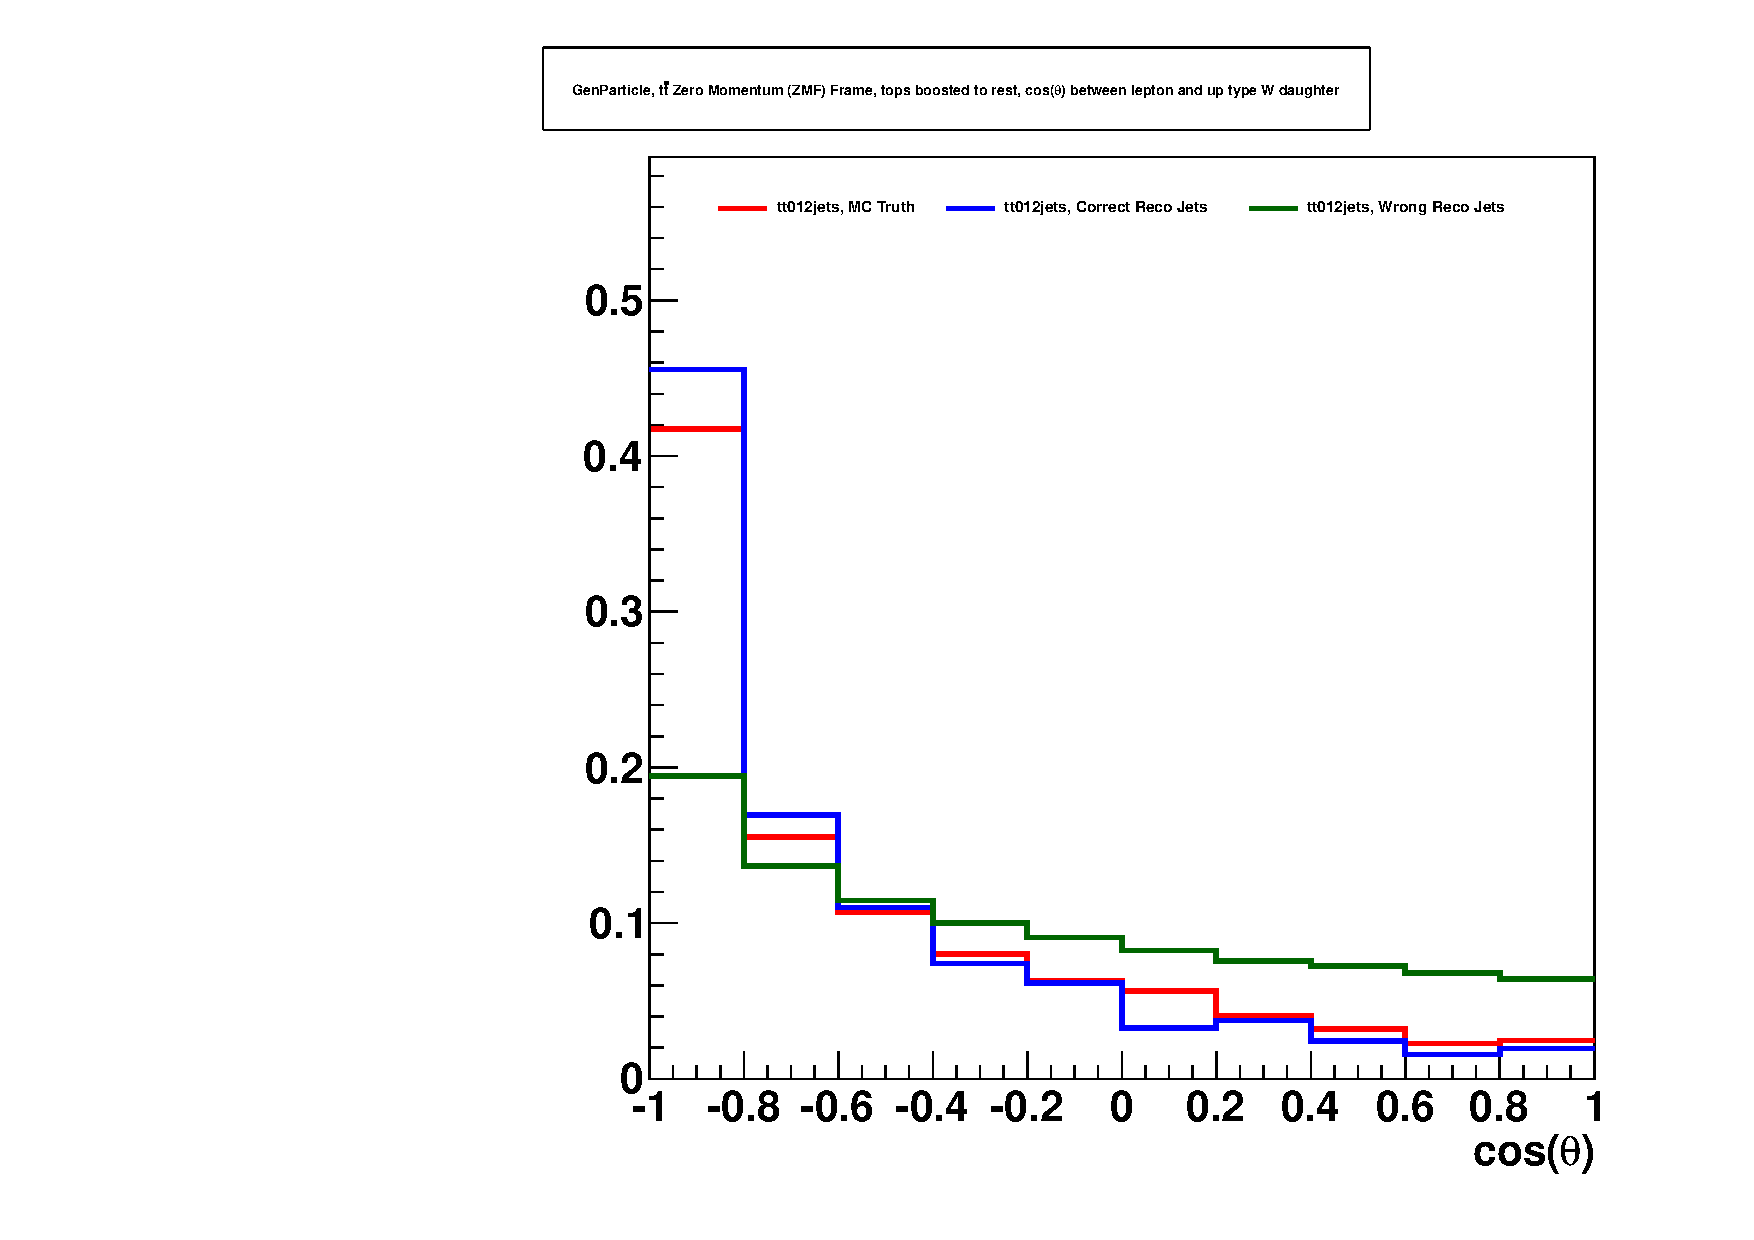
\includegraphics[width=0.31\textwidth]{Figures/Analysis_Improvement_Diagrams/tt012jets__h_genParticle_ttbarZMFrame_topsRest_cos3dPolarAngle_lep_hadWupQ__vs__h_recoJets_correctAssoc_ttbarZMFrame_topsRest_cos3dPolarAngle_lep_hadWupQ__vs__h_recoJets_wrongAssoc_ttbarZMFrame_topsRest_cos3dPolarAngle_lep_hadWupQ__unitNorm.pdf}
    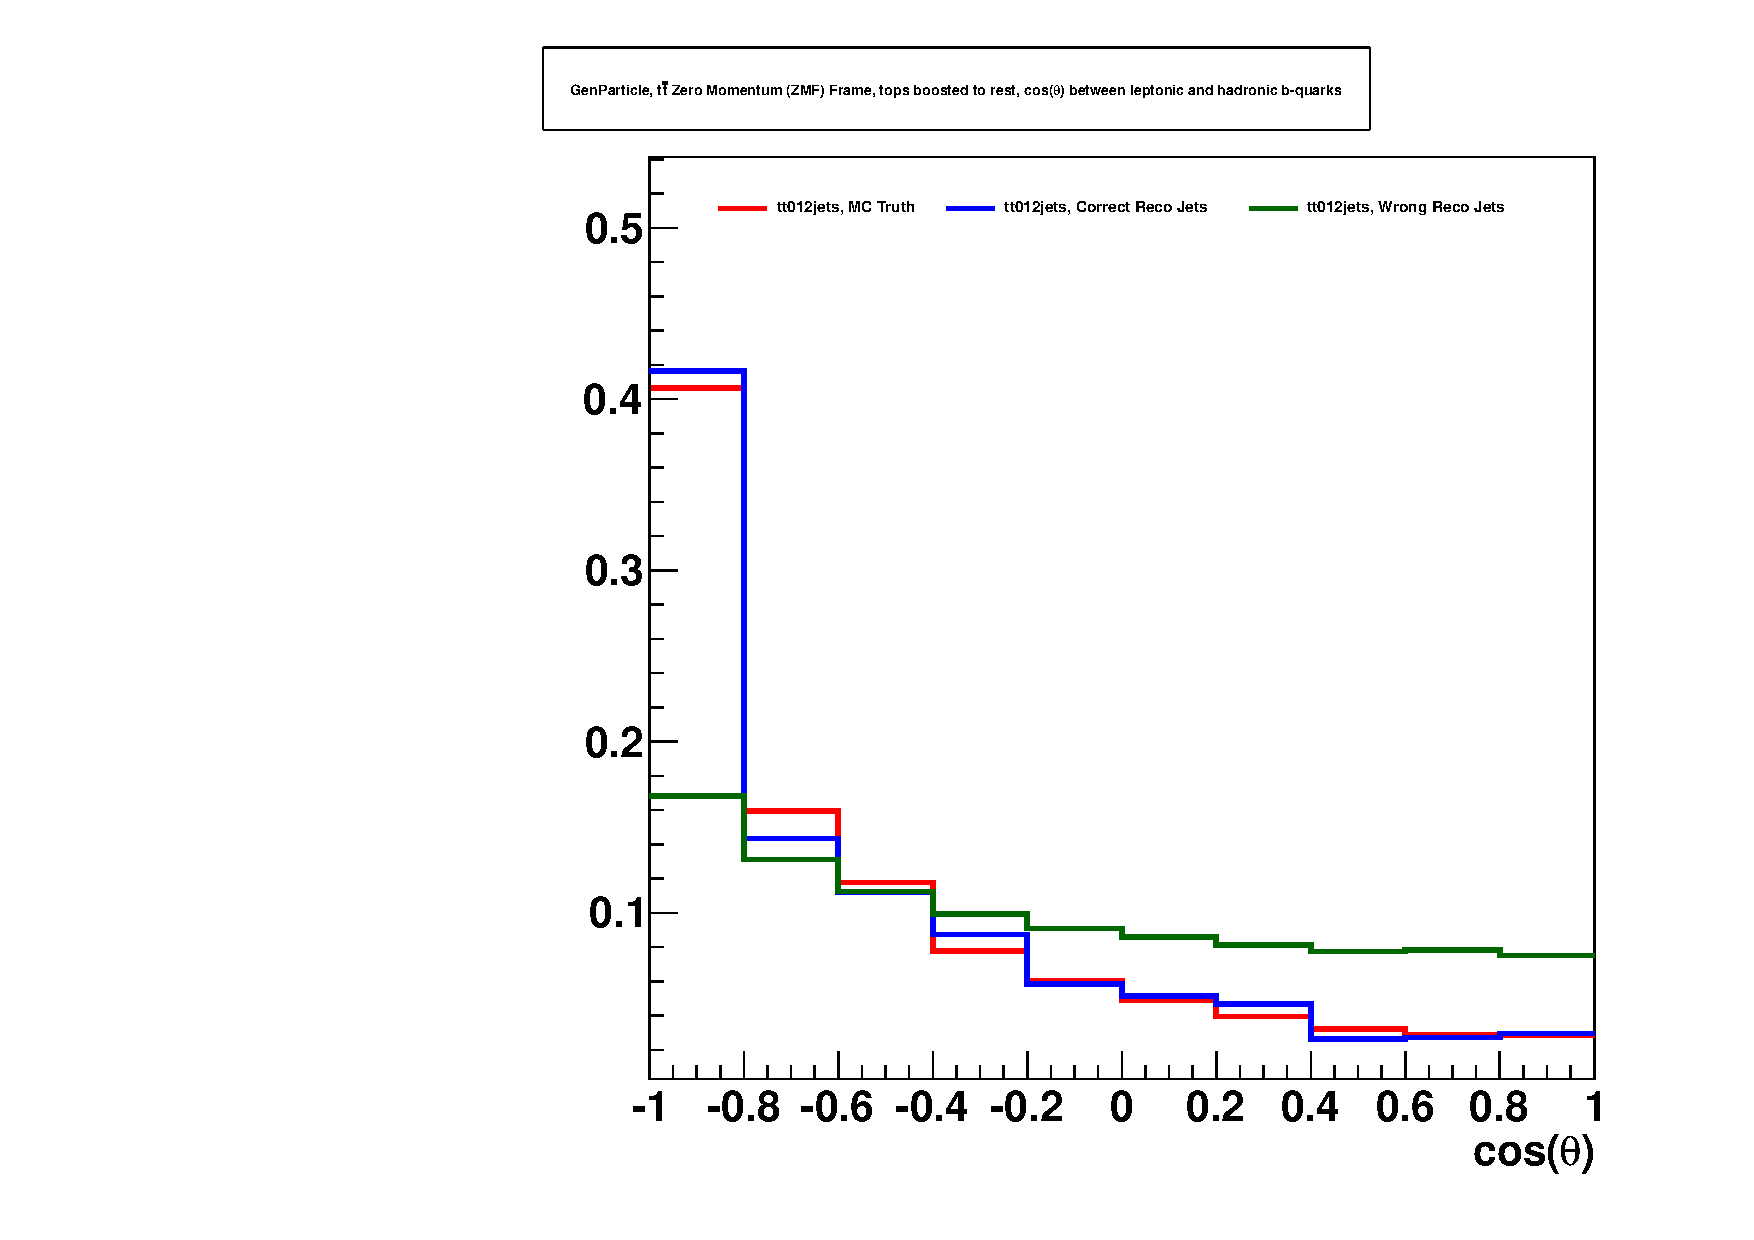
\includegraphics[width=0.31\textwidth]{Figures/Analysis_Improvement_Diagrams/tt012jets__h_genParticle_ttbarZMFrame_topsRest_cos3dPolarAngle_lepB_hadB__vs__h_recoJets_correctAssoc_ttbarZMFrame_topsRest_cos3dPolarAngle_lepB_hadB__vs__h_recoJets_wrongAssoc_ttbarZMFrame_topsRest_cos3dPolarAngle_lepB_hadB__unitNorm.pdf}
    \caption{The cosine of the anlge between the momentum
      three-vectors for the $b$-quarks from the top decays (left), the
    lepton and the up-type $W$ boson daughter (center), and the lepton
  and the down-ype $W$ boson daughter (right)}
    \label{fig:aMCatNLO_cos3dPolar}}
\end{figure}

\noindent All three distributions have peaking values that provide
discrimination between the jets correctly associated to the MC truth
generator-level partons of the \ttbar decay, and the jets which are
incorrectly associated.  In each plot, the green represents the
incorrect associations, while the blue represents the correct
associations, and the red represents the MC truth from the generated
parton.  An additional angle of interest is the difference in the
$\phi$ coordinate between daughters of the \ttbar decay.  Figure
\ref{fig:aMCatNLO_deltaPhi} shows the distributions for the
$\Delta\phi$ between the $b$-quarks from the top decays, the lepton
and up-type $W$-boson daughter, and the lepton and the down-type
$W$-boson daughter.  The case of the correctly associated jets has two
sharp peaks near $\phi = \pm 2$, where the distribution is more
uniform for incorrectly associated jets.  

\begin{figure}[hbtp] 
  {\centering
    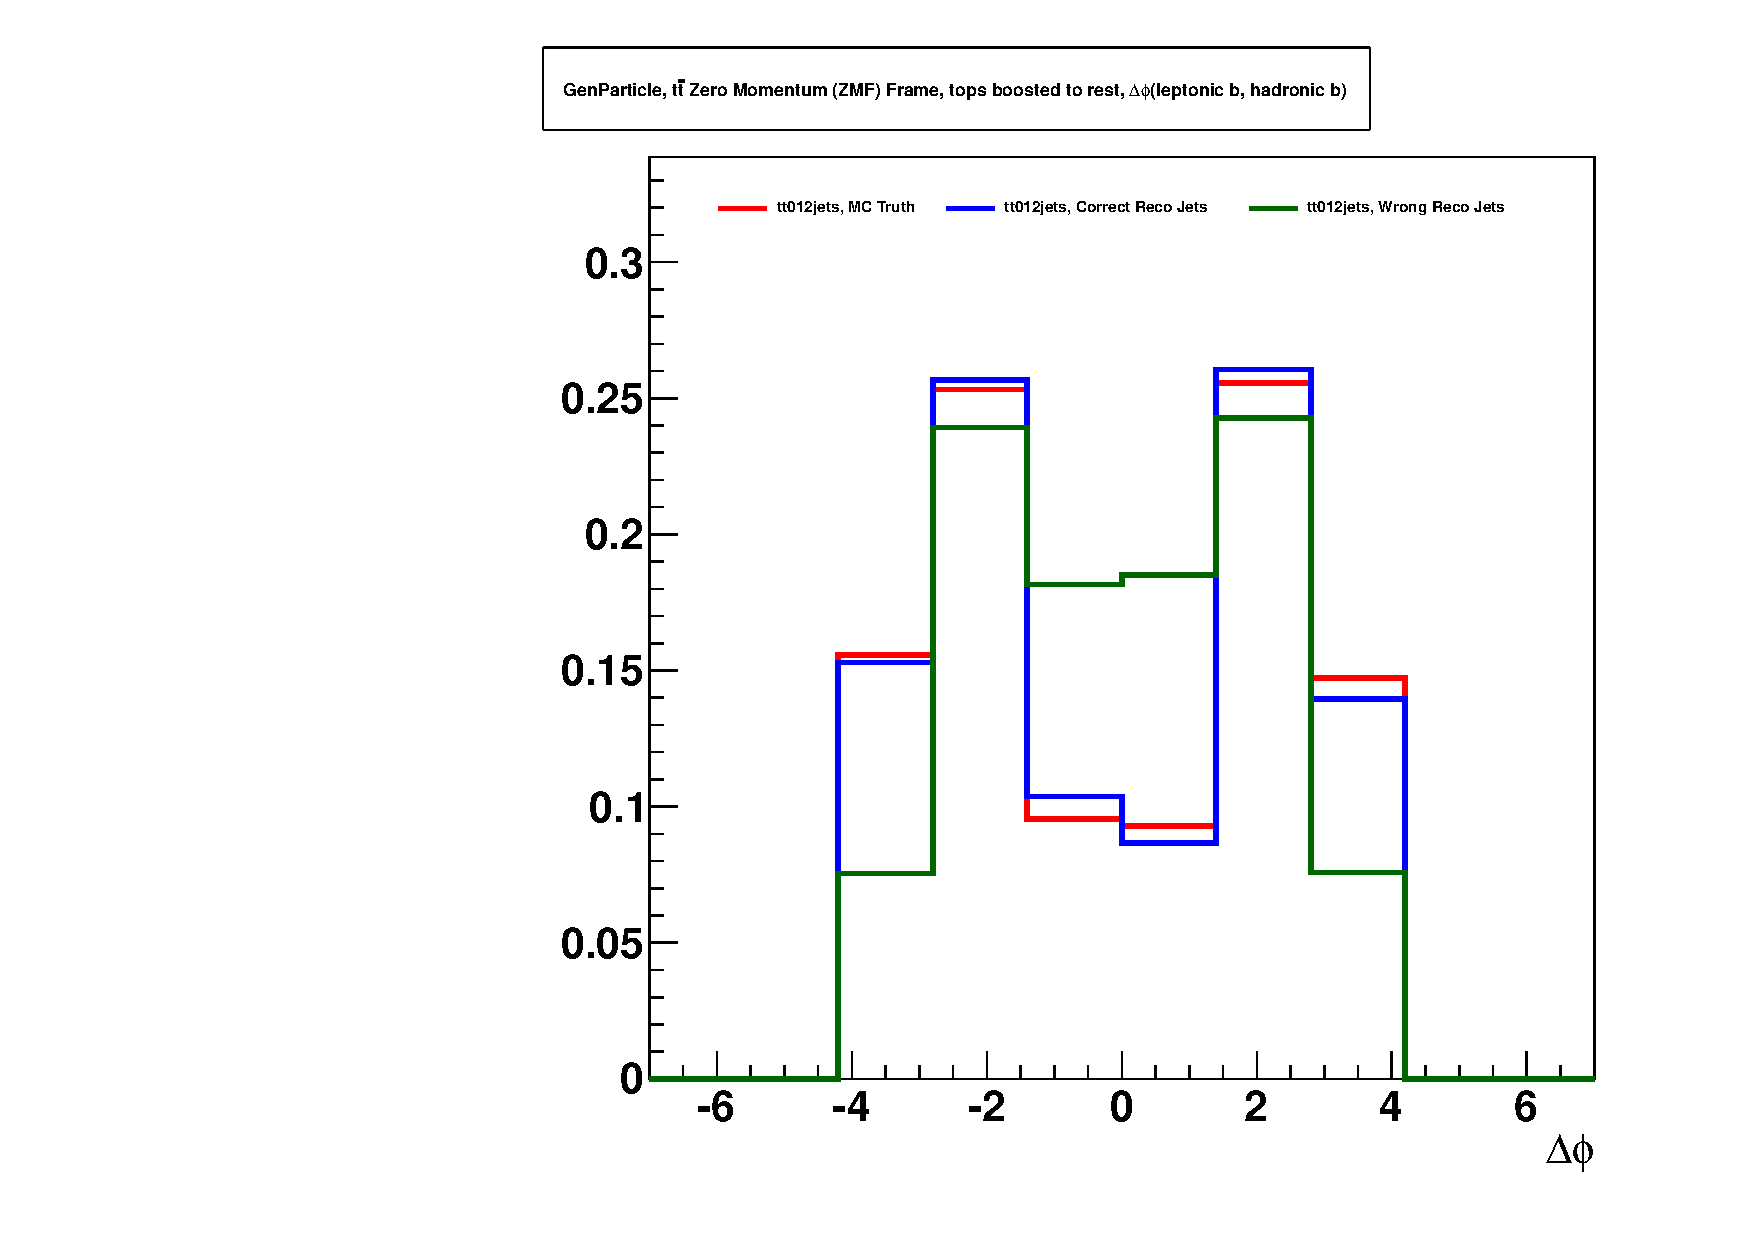
\includegraphics[width=0.31\textwidth]{Figures/Analysis_Improvement_Diagrams/tt012jets__h_genParticle_ttbarZMFrame_topsRest_deltaPhi_lepB_hadB__vs__h_recoJets_correctAssoc_ttbarZMFrame_topsRest_deltaPhi_lepB_hadB__vs__h_recoJets_wrongAssoc_ttbarZMFrame_topsRest_deltaPhi_lepB_hadB__unitNorm.pdf}
    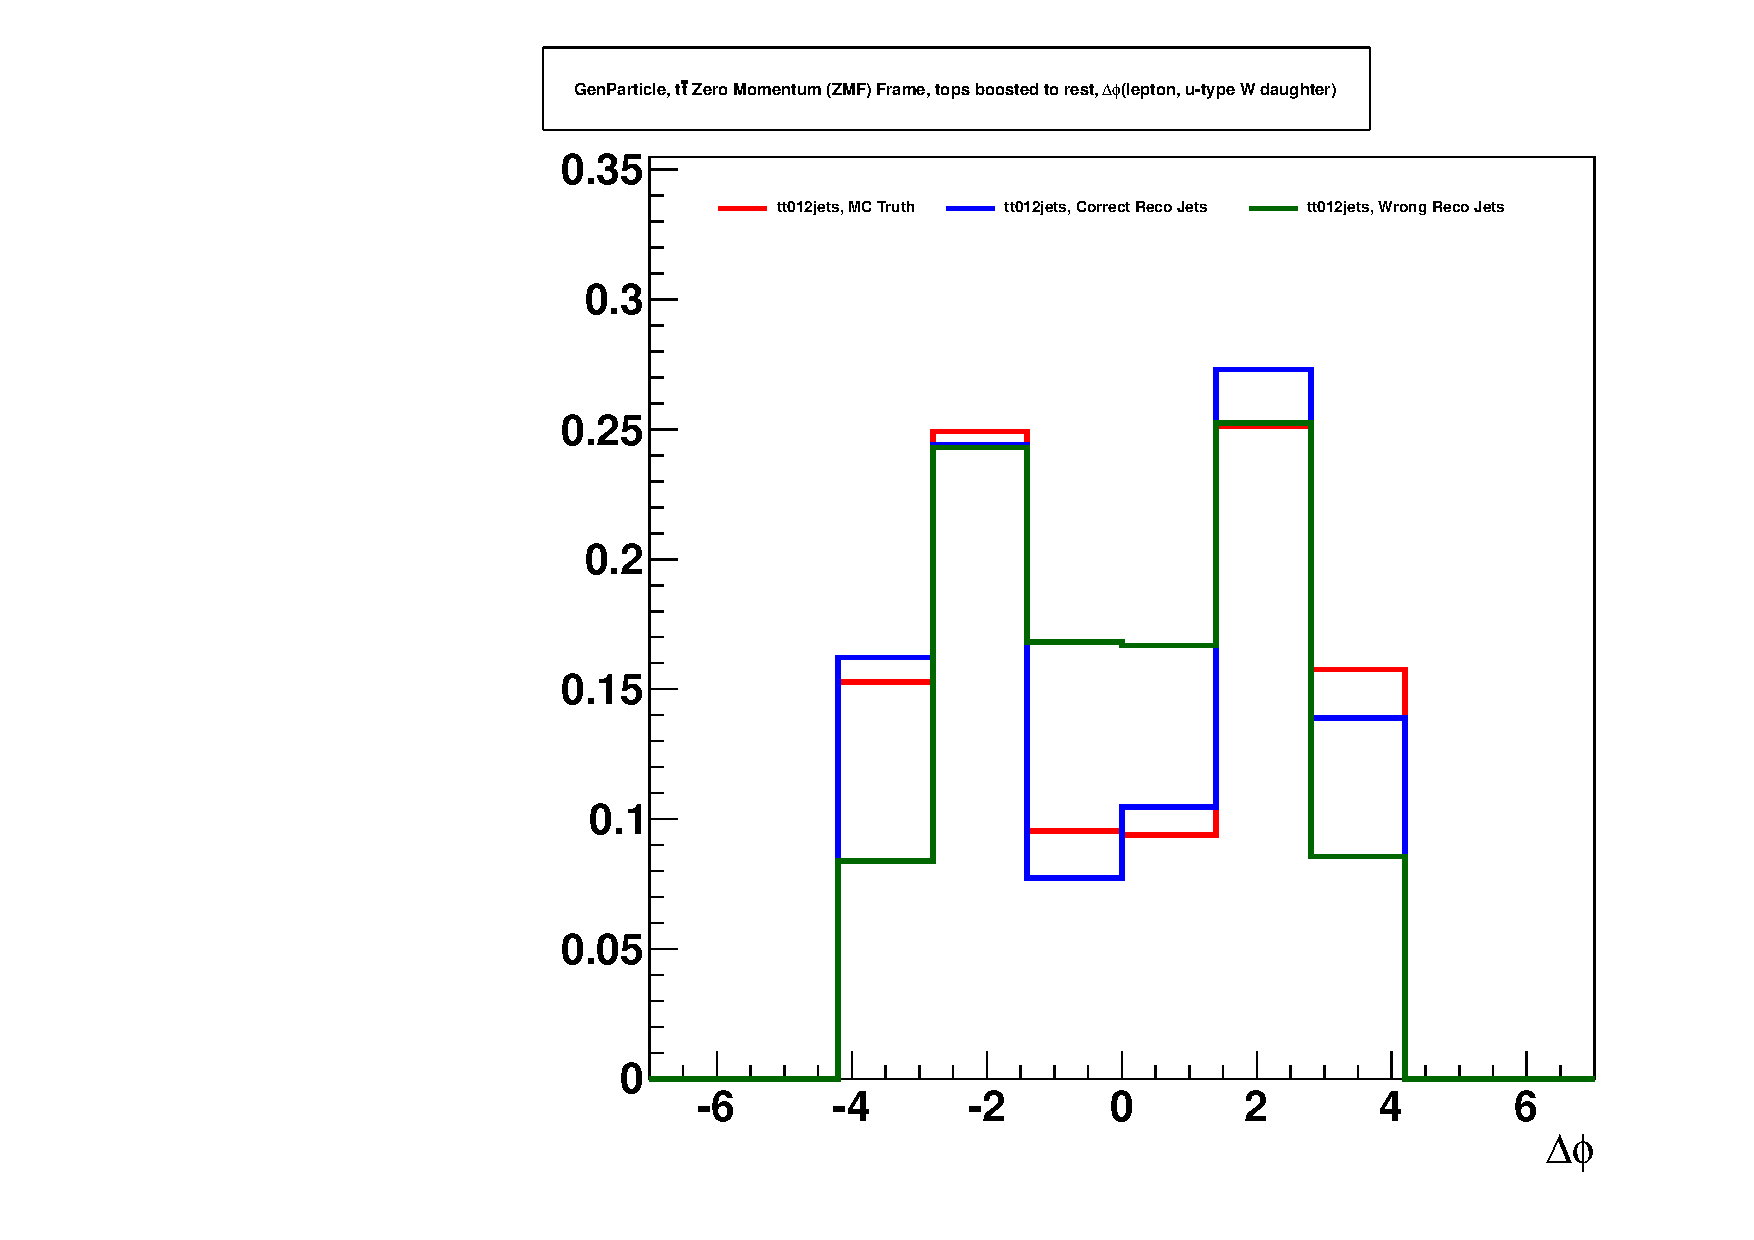
\includegraphics[width=0.31\textwidth]{Figures/Analysis_Improvement_Diagrams/tt012jets__h_genParticle_ttbarZMFrame_topsRest_deltaPhi_lep_hadWupQ__vs__h_recoJets_correctAssoc_ttbarZMFrame_topsRest_deltaPhi_lep_hadWupQ__vs__h_recoJets_wrongAssoc_ttbarZMFrame_topsRest_deltaPhi_lep_hadWupQ__unitNorm.pdf}
    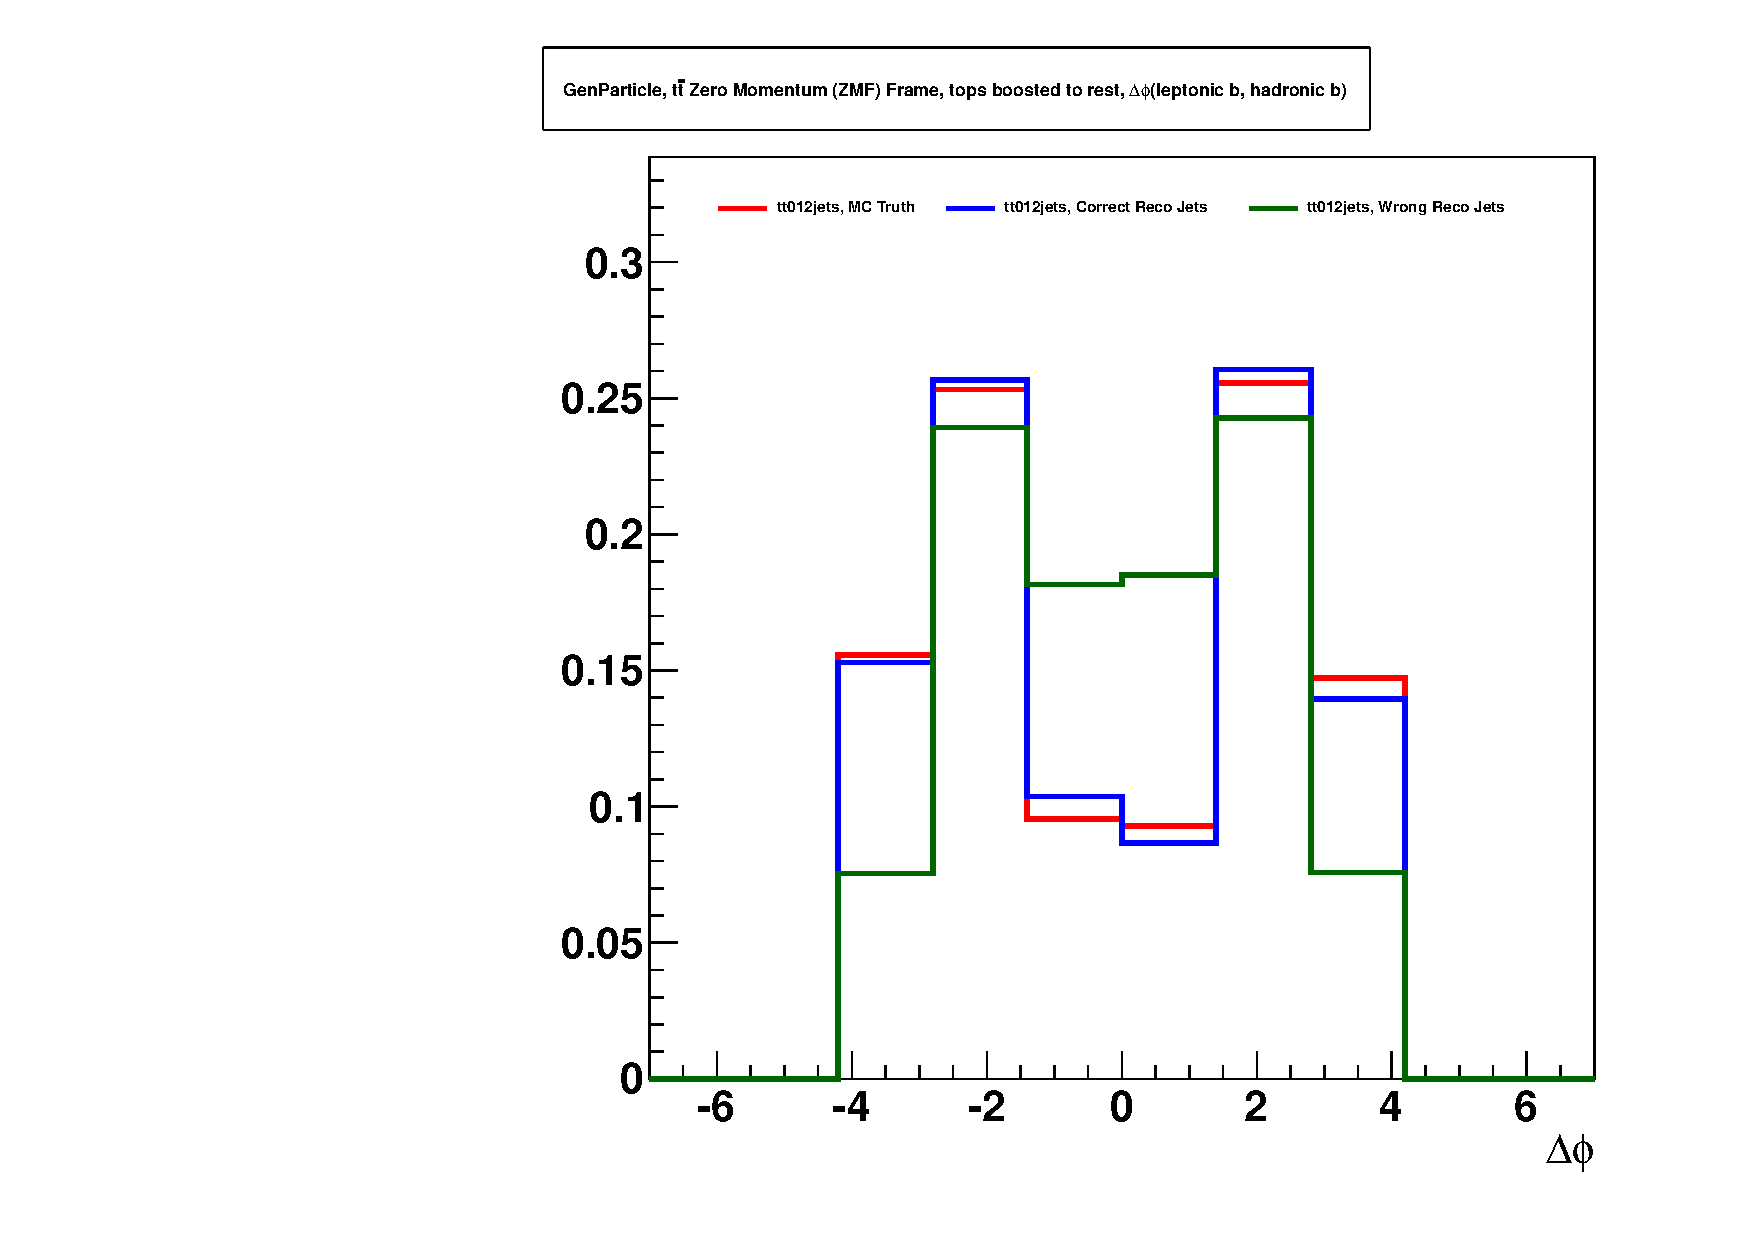
\includegraphics[width=0.31\textwidth]{Figures/Analysis_Improvement_Diagrams/tt012jets__h_genParticle_ttbarZMFrame_topsRest_deltaPhi_lepB_hadB__vs__h_recoJets_correctAssoc_ttbarZMFrame_topsRest_deltaPhi_lepB_hadB__vs__h_recoJets_wrongAssoc_ttbarZMFrame_topsRest_deltaPhi_lepB_hadB__unitNorm.pdf}
    \caption{The difference in the $\phi$ coordinate between the momentum
      three-vectors for the $b$-quarks from the top decays (left), the
    lepton and the up-type $W$ boson daughter (center), and the lepton
  and the down-ype $W$ boson daughter (right)}
    \label{fig:aMCatNLO_deltaPhi}}
\end{figure}

\par A final variable of interest for jet association would be the
charge of lepton multiplied against the charge of the $b$-quark that
is associated with the same top-quark.  These two values, due to
charge conservation, will always be negative when multiplied.  The
charge of the jet is calculated from a \PT weighted sum of the tracks
contained in the cluster, where the curvature of each track tells the
charge of the hadron creating the signature.  Since there are many
hadrons clustered together to form a jet, there is a large degradation
on resolution of the charge of the jet, however for the peak of this
distrubtion is negative for correctly associated jets, and positive
for incorrect jets, as shown in figure
\ref{fig:aMCatNLO_lepJetCharge}.  

\begin{figure}[hbtp] 
  {\centering
    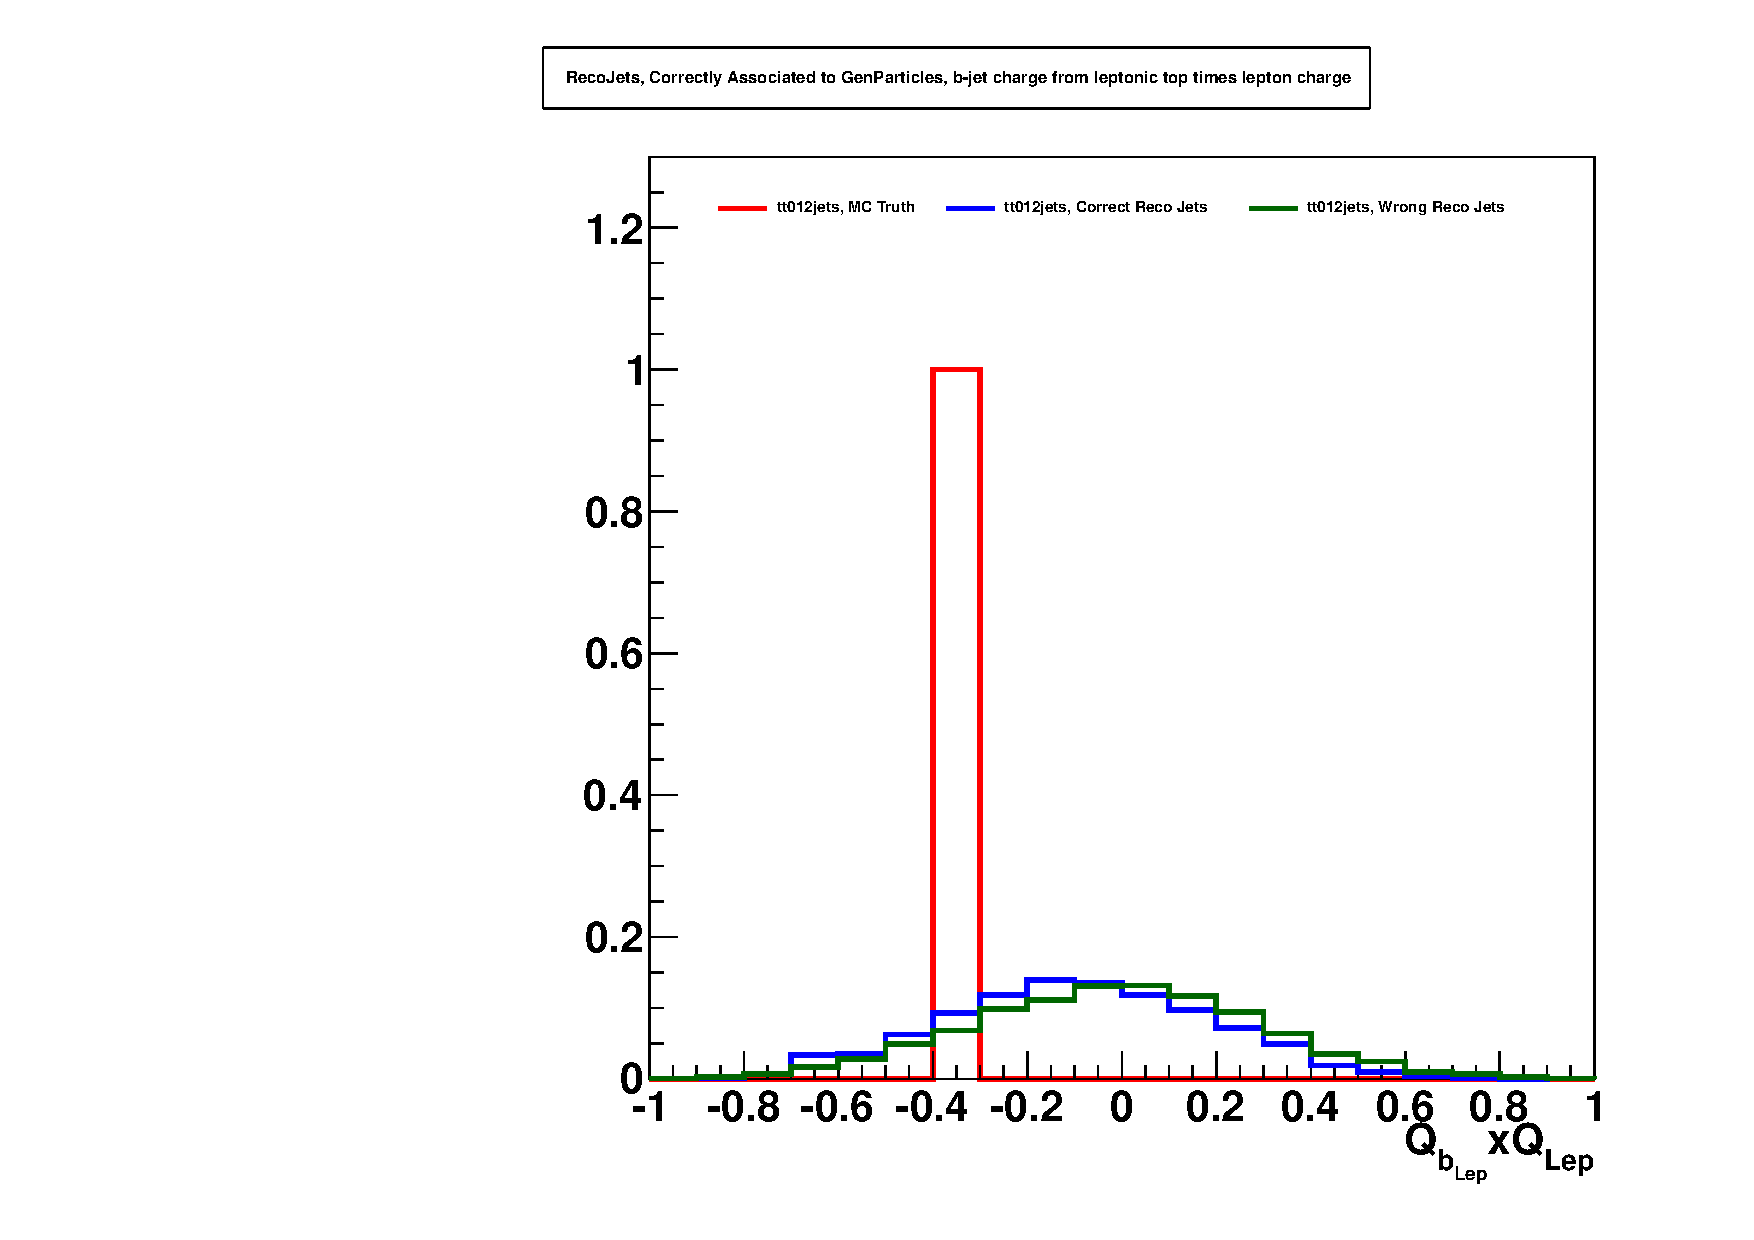
\includegraphics[width=0.50\textwidth]{Figures/Analysis_Improvement_Diagrams/tt012jets__h_genParticle_lepBChargeLepCharge__vs__h_recoJets_correctAssoc_labFrame_lepBChargeLepCharge__vs__h_recoJets_wrongAssoc_labFrame_lepBChargeLepCharge__unitNorm.pdf}
    \caption{Jet times lepton charge, for the $b$-jet associated with
      the same top as the lepton.  Green shows incorrectly associated
      reconstructed jets, blue shows correctly associated jets, and
      red is the MC truth}
    \label{fig:aMCatNLO_lepJetCharge}}
\end{figure}

\par  A jet association algorithm can be formed by using an MVA
technique to provide a discriminant for how likely a certain
combination of jets from an event are correctly associated to their
roles in the decay of the \ttbar system.  A training sample of
correctly and incorrectly associated jets can be trained using the
following variables:

\begin{itemize}
  \item Invariant Mass of the Hadronic $W$ boson
  \item Invariant Mass of the Leptonic $W$ boson
  \item Invariant Mass of the Hadronic top-quark
  \item Invariant Mass of the Leptonic top-quark
  \item $\cos{\theta_{b, \bar{b}}}$ in the frame where $\ttbar$ system and
    $t$-quarks are at rest respectively 
  \item $\cos{\theta_{lep, up-type W daughter}}$ in the frame where $\ttbar$ system and
    $t$-quarks are at rest respectively 
  \item $\cos{\theta_{lep, down-type W daughter}}$ in the frame where $\ttbar$ system and
    $t$-quarks are at rest respectively 
  \item $\Delta\phi(\theta_{b, \bar{b}})$ in the frame where $\ttbar$ system and
    $t$-quarks are at rest respectively 
  \item $\Delta\phi(\theta_{lep, up-type W daughter})$ in the frame where $\ttbar$ system and
    $t$-quarks are at rest respectively 
  \item $\Delta\phi(\theta_{lep, down-type W daughter})$ in the frame where $\ttbar$ system and
    $t$-quarks are at rest respectively 
   \item The product of the lepton and $b$-quark associated with the
     same $t$-quark
\end{itemize}


\par  An additional improvement to the analysis will rely on a
dedicated MVA for each of the \ttbar+X backgrounds, where X is light
flavor, single $c$, $c\bar{c}$, single $b$, and $b\bar{b}$.  A
dedicated \ttbb and even a \ttcc sample with sufficiently large enough
events to train an MVA would be ideal.  The discrimiants from each of
the backgrounds would be combined as input variables to a second MVA,
in order to produce a discriminant for how likely the event is from a
\ttH decay.  

